\documentclass[a4paper]{article}

\usepackage{pgfplots}

\pgfplotsset{compat=1.5}
\begin{document}

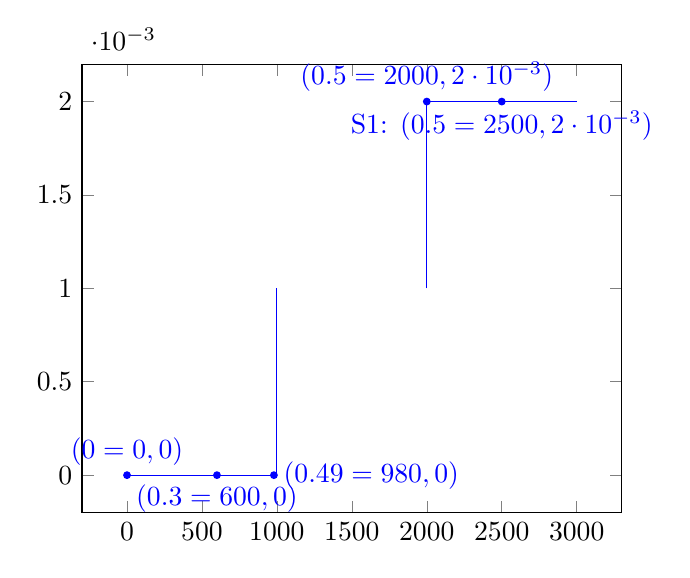
\begin{tikzpicture}
\tikzset{drawit/.style={circle,inner sep=1pt,fill=blue}}
%\tracingmacros=2 \tracingcommands=2
	\begin{axis}[%axis equal,
		clip=false,/pgf/number format/1000 sep={{{}}}
	]
	\addplot[blue] coordinates {(0,0) (1000,0) (1000,1e-3) 
	
		(2e3,1e-3) (2e3,2e-3) (3e3,2e-3)
	}
		node[pos=0,drawit] {}
		node[pos=0,above] {%
			\pgfplotspointplotattime%
			$(0=
			\pgfmathprintnumber{\pgfkeysvalueof{/data point/x}},
			\pgfmathprintnumber{\pgfkeysvalueof{/data point/y}}
			)$%
		}
		node[pos=0.3,drawit] {}%
		node[pos=0.3,below] {%
			\pgfplotspointplotattime%
			$(0.3=
			\pgfmathprintnumber{\pgfkeysvalueof{/data point/x}},
			\pgfmathprintnumber{\pgfkeysvalueof{/data point/y}}
			)$%
		}
		node[pos=0.49,drawit] {}%
		node[pos=0.49,anchor=west] {%
			\pgfplotspointplotattime%
			$(0.49=
			\pgfmathprintnumber{\pgfkeysvalueof{/data point/x}},
			\pgfmathprintnumber{\pgfkeysvalueof{/data point/y}}
			)$%
		}
		node[pos=0.5,drawit] {}%
		node[pos=0.5,above] {%
			\pgfplotspointplotattime%
			$(0.5=
			\pgfmathprintnumber{\pgfkeysvalueof{/data point/x}},
			\pgfmathprintnumber{\pgfkeysvalueof{/data point/y}}
			)$%
		}
		node[pos=0.5,pos segment=1,drawit] {}%
		node[pos=0.5,pos segment=1,below] {%
			\pgfplotspointplotattime%
			S1: 
			$(0.5=
			\pgfmathprintnumber{\pgfkeysvalueof{/data point/x}},
			\pgfmathprintnumber{\pgfkeysvalueof{/data point/y}}
			)$%
		}
	;	
	\end{axis}
\end{tikzpicture}
\end{document}

